\documentclass{article}

\usepackage[margin=1in]{geometry}
\usepackage[utf8]{inputenc}
\usepackage[english]{babel}
\usepackage{amsthm} %lets us use \begin{proof}
\usepackage{amssymb} %gives us the character \varnothing
\usepackage{xcolor}
\usepackage{float}
\usepackage{braket}
\usepackage{multirow}
\usepackage{array}
\usepackage{mathtools}

\title{Chem150L: Final} % Title of the assignment

\begin{document}

\maketitle

\section*{Electronic Structure of a New Carborane Radical}

\noindent a) Perform an initial geometry optimization of \textit{meta}-C$_2$B$_{10}$H$_{11}$
using def2-SV(P) basis sets and TPSS/RI. (8)
\\

{\color{blue} Performed geometry optimization and verified.}
\\

\noindent b) Confirm that the converged structure is a minimum by analytical
second derivative calculations. What point group symmetry, if any, does the
radical have? (4)
\\

{\color{blue} $C_s$ point group symmetry.}

\begin{figure}[H]
  \centering
  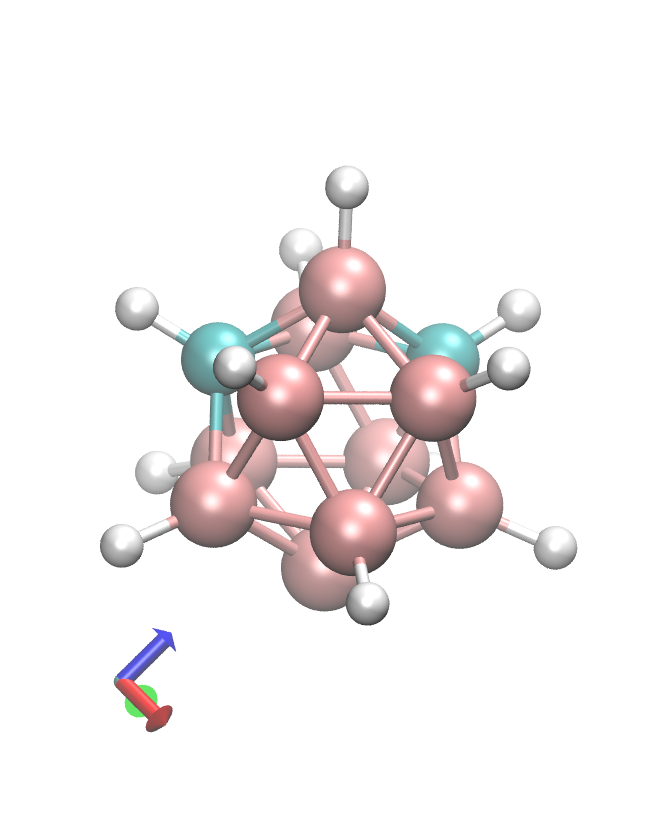
\includegraphics[scale=0.25]{opt.png}
  \caption{Geometry optimized \textit{meta}-C$_2$B$_{10}$H$_{11}$ with
    RI-TPSS/def2-SV(P) basis sets.}
\end{figure}

\noindent c) Refine the structure by re-optimizing it using def2-TZVP basis
sets and the TPSSh. Use the refined methodology for the following property
calculations. (4)
\\

{\color{blue} Performed geometry optimization and verified.}
\\

\noindent d) Investigate the bonding in the cluster core by visually inspecting
the orbitals and their energies. Identify and plot the low-lying totally symmetric
delocalized valence orbital expected from the Wade rules. Can the electronic
structure of the radical be described by localized two-electron two-center
bonds? (4)

\begin{figure}[H]
  \centering
  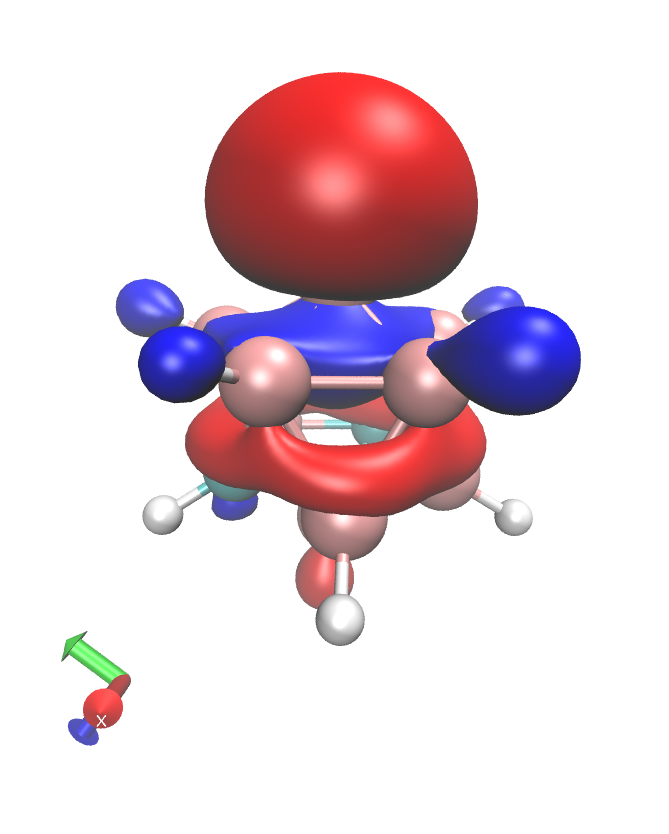
\includegraphics[width=0.3\textwidth]{homo_37a_a.png}
  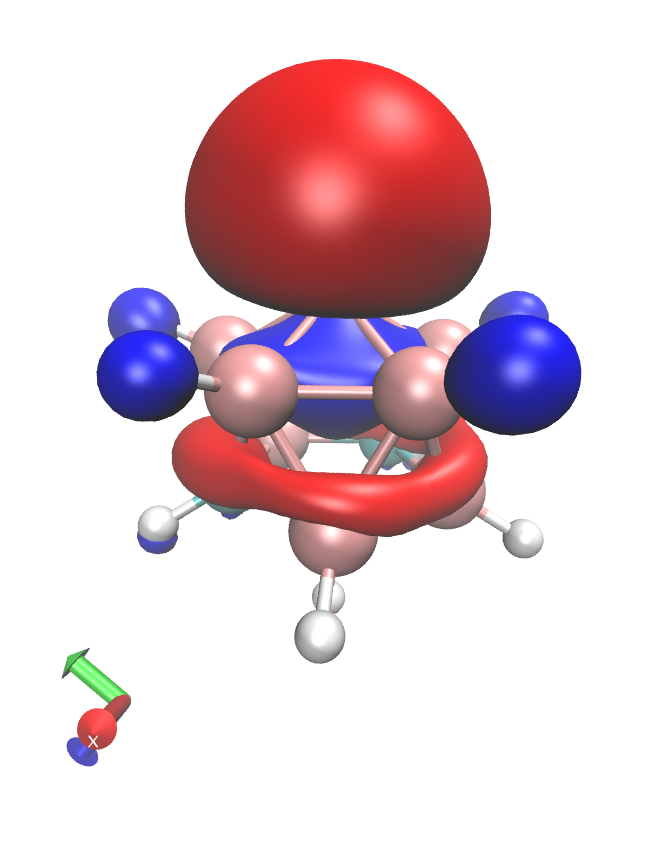
\includegraphics[width=0.3\textwidth]{lumo_37a_b.png}
  \caption{Molecular orbitals of the HOMO (left) and LUMO (right) for
    \textit{meta}-C$_2$B$_{10}$H$_{11}$. HOMO energy is $-5.18$ eV and
    LUMO energy is $-2.36$ eV.}
  \label{fig:orbital}
\end{figure}

\noindent e) Perform a population analysis of the spin density and plot
it in 3 dimensions. Do your results support the hypothesis of a boron-centered,
localized radical? (4)

\begin{figure}[H]
  \centering
  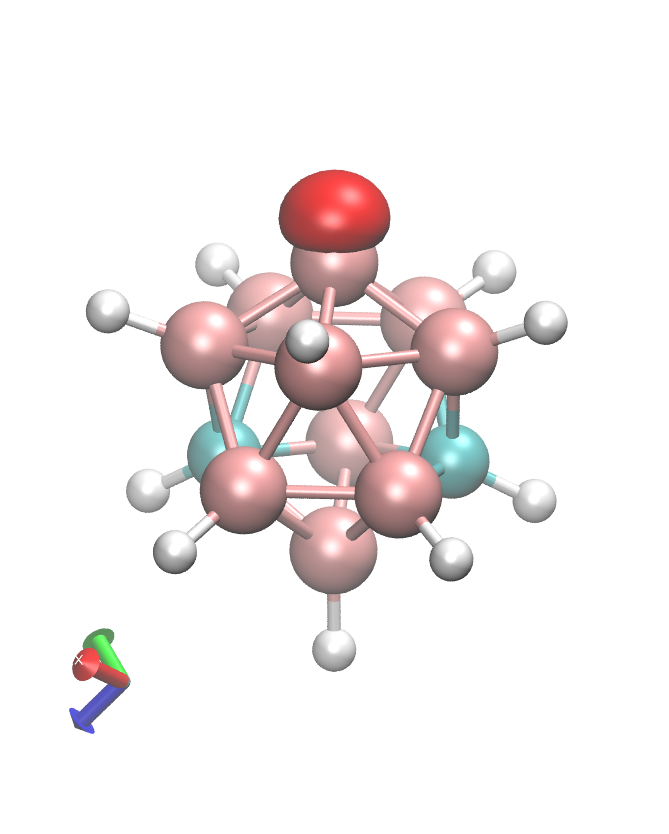
\includegraphics[scale=0.35]{spin_dens.png}
  \caption{Spin density of the \textit{meta}-C$_2$B$_{10}$H$_{11}$.}
  \label{fig:spin}
\end{figure}

{\color{blue} Population analysis of the spin density on the boron without
  the terminal hydrogen is given in Table \ref{tab:pop}. Yes, the population
  analysis and the spin density plot support the hypothesis of a boron-centered,
  localized radical.
}

\begin{table}[H]
  \centering
  \caption{Population analysis of the spin-unrestricted calculation
    for the spin density ($D^{\alpha}-D^{\beta}$) for the boron with the
    terminal hydrogen in \textit{meta}-C$_2$B$_{10}$H$_{11}$.}
  \begin{tabular}{ccccc}
    Atom & Total & n(s) & n(p) & n(d) \\
    \hline
    B & 0.834 & -0.022 & 0.846 & 0.011
  \end{tabular}
  \label{tab:pop}
\end{table}

\noindent f) Investigate the redox chemistry of the radical by computing
the first vertical ionization potential and electron affinity (using
self-consistent energy calculations for the cation and the anion). (4)
\\

\begin{table}[H]
  \centering
  \caption{Ionization potential and electron affinity
    reported in eV.}
  \begin{tabular}{ccc}
    Molecule & Ionization Potential & Electron Affinity \\
    \hline
    \textit{meta}-C$_2$B$_{10}$H$_{11}$ & 7.744 & 0.495 \\
  \end{tabular}
  \label{tab:ip_affinity}
\end{table}


\noindent g) Simulate and plot the low-energy UV spectrum by computing the
first 10 dipole-allowed excitations and broadening the obtained oscillator
strengths with Gaussians using 0.16 eV linewidth. Hint: Specifying the data
group \texttt{\$spectrum nm} in the control file will result in a separate file spectrum
containing the excitation energies and oscillator strengths. Assign the
lowest-energy band in the spectrum based on the dominant occupied-unoccupied
orbital pairs involved in the underlying transition. (8)
\\


\end{document}
